% ==========================================
% LatexRefinement Step Output: step4-04-28-25-tuesday-all-offset-final.tex
% Model: gemini-3-flash-preview
% Temperature: 0.36
% TopP: 0.95
% TopK: 40
% MaxOutputTokens: 65535
% ThinkingBudget: 32765
% ThinkingLevel: HIGH
% Prompt Tokens: 35'650
% Candidates Tokens: 18'915 (inkl. Thinking Tokens)
% Cached Tokens: 0
% Processed on: 2026-07-11 12:20:54
% ==========================================

\lecturechapter{Dienstag}{28. Apr}{28. April 2026}{Einführung in die Graphentheorie}

\begin{nice-box}[Kontext der Vorlesung \& Syllabus]
In dieser Vorlesung beginnen wir mit einem neuen großen Thema: der Graphentheorie. Nach dem Abschluss des Kapitels über das Auswahlaxiom und Kardinalzahlen lassen wir die formalen Logikstrukturen vorerst hinter uns und widmen uns den anschaulichen, diskreten Strukturen der Graphen.

\textbf{Syllabus:}
\begin{enumerate}[label=\textbf{(\arabic*)}]
    \item \textbf{Historischer Kontext:} Leonhard Euler und das Königsberger Brückenproblem.
    \item \textbf{Grundbegriffe:} Formale Definition von Graphen, Knoten, Kanten und Adjazenz.
    \item \textbf{Graphentypen:} Gerichtete vs. ungerichtete Graphen, Schlingen, Mehrfachkanten und schlichte Graphen.
    \item \textbf{Adjazenzmatrix:} Matrixdarstellung von Graphen und ihre Eigenschaften.
    \item \textbf{Knotengrade:} Definition des Grades in Digraphen (Halbgrade) und ungerichteten Graphen.
    \item \textbf{Spezielle Graphen:} Reguläre Graphen, vollständige Graphen ($K_n$) und Teilgraphen.
    \item \textbf{Pfade und Züge:} Definition von Pfeilzügen, Bahnen, Wirbeln, Kantenzügen, Wegen und Kreisen.
    \item \textbf{Kombinatorik:} Pfadzählung mittels Potenzen der Adjazenzmatrix.
\end{enumerate}
\end{nice-box}

\section{Einführung und historischer Kontext}

\begin{spoken-clean}[00:00:00 - 00:01:07]
Okay, hallo. Hallo zusammen und herzlich willkommen zur nächsten Woche von Grundstrukturen.

Wie ich das letzte Mal gesagt habe, schließen wir das Kapitel über das Auswahlaxiom und Kardinalzahlen jetzt ab. Im Skript sehen Sie dazu noch zwei Kapitel über Nichtstandard-Analysis; die werden wir überspringen. Die sind \qt{nicht so standard}, aber es ist ein witziges Thema, falls Sie Lust haben, dort einmal reinzuschauen.

Es geht darum, Nichtstandard-Modelle der reellen Zahlen zu konstruieren. Auf diesen Nichtstandard-Modellen kann man dennoch Analysis betreiben und diese Modelle dann wiederum verwenden, um Aussagen über die Standard-Analysis zu treffen. Es ist ein lustiges Thema. Ja?
\end{spoken-clean}

\begin{student-interaction}[Studentenfrage]
Wenn wir das überspringen, ist das dann noch examensrelevant?
\end{student-interaction}

\begin{spoken-clean}[00:01:07 - 00:01:25]
Nein, es ist nicht examensrelevant. Das Skript ist etwas länger als eine zweistündige Vorlesung, deswegen darf da jeder ein bisschen seine Auswahl treffen. Vielleicht werden wir noch ein paar Sachen machen, die nicht im Skript stehen; die werde ich Ihnen dann aber dazu geben.

Schauen Sie sich das ruhig an, wenn Sie sich für diese Sachen interessieren. Das ist lustig, und Sie können dazu auch noch weiterlesen, zum Beispiel im Buch von Lorenz Halbeisen und Regula Krapf.
\end{spoken-clean}

\begin{spoken-clean}[00:01:25 - 00:03:08]
Wir machen jetzt direkt weiter im Kapitel über die Graphentheorie. Damit lassen wir vorerst auch einmal diese Logikgeschichten zurück --- obwohl man die natürlich nie ganz zurücklässt, weil die gesamte Mathematik auf der Logik und auf Zermelo-Fraenkel aufbaut. Im Hintergrund verwenden wir diese ganzen Sachen natürlich immer noch: Man kann sich weiterhin Signaturen anschauen und das Ganze entsprechend formulieren. Man kann auch alle Beweise, die wir führen, formalisieren und auf Zermelo-Fraenkel zurückführen. Das ist etwas, was Leute machen, zum Beispiel mit der Sprache \emph{Lean}.

Um jedoch einigermaßen voranzukommen, werden wir die Dinge jetzt in --- wie soll ich sagen --- alltäglicher mathematischer Sprache diskutieren. Es geht also darum, dass Sie ein paar Grundbegriffe lernen: jetzt eben ein bisschen sehr elementare Graphentheorie, danach noch etwas sehr elementare Zahlentheorie, wahrscheinlich auch noch etwas über endliche Körper und, wenn wir Zeit haben, noch ein bisschen elementare Gruppentheorie.

Das dient einfach dazu, dass Sie gewisse Sachen lernen, für die Sie in anderen Vorlesungen keine Zeit haben, und damit Sie einen Einblick kriegen in das, was es in der Mathematik so alles gibt. Auch hier ist es überall wieder wichtig, dass Sie die Übungen lösen, denn es geht darum, dass Sie lernen, saubere mathematische Argumente zu führen --- das ist es, was Sie am Ende können sollten.
\end{spoken-clean}

\begin{spoken-clean}[00:03:08 - 00:05:40]
Gut, jetzt aber zur Graphentheorie. Ein bisschen Geschichte: Da gehen wir jetzt etwas weiter zurück als zu den Leuten, denen wir bisher begegnet sind. Wir gehen zurück zu Leonhard Euler, dem Sie bestimmt auch schon begegnet sind. Er war gewissermaßen ein Schweizer Mathematiker --- er wurde $1707$ in Basel geboren. Das war also noch sehr früh in der Mathematik.

Damals, gab es natürlich noch keine ETH, aber es gab schon seit Langem die Universität Basel; das ist auch der Ort, an dem er studiert hat. Zu jener Zeit waren die Bernoullis an der Uni Basel. Das ist eine ganze Familiengeneration, die über mehrere Generationen hinweg denselben Lehrstuhl innehatte. Sie waren sehr einflussreich in der Entwicklung der Mathematik und der Physik.

Euler ging damals, ich glaube Samstagnachmittags, zu Johann Bernoulli, der ihm dann ein paar Sachen erklärte. Ich glaube, Johann Bernoulli hatte nicht viel Zeit; er hat ihm viele Sachen zu lesen gegeben. Aber Euler hat einmal geschrieben, dass es wunderbar war: Er hat oft nur wenige Fragen gestellt, und die Art und Weise, wie Bernoulli ihm diese Sachen beantwortet hat, hat ihm sofort auch viele andere Fragen geklärt.

Euler hat sich, glaube ich, auch für eine Physikprofessur in Basel beworben, die er aber nicht kriegte, weil er noch sehr jung war. Dann ist er halt weggegangen und leider akademisch nie mehr in die Schweiz zurückgekehrt. Er hat dann eine Professur in Sankt Petersburg bekommen --- ich glaube, damals war noch ein anderer Bernoulli dort ---, war dann eine Zeit lang in Berlin und schließlich wieder in Sankt Petersburg.

Ich glaube, man kann fast nicht unterschätzen, wie wichtig Euler für viele moderne Begriffe in der Mathematik war; er hat viele Gebiete eigentlich fast neu erfunden. Eines davon ist die Graphentheorie. Es begann mit dem folgenden Problem --- gewissermaßen war das vielleicht sogar die Erfindung der Topologie.
\end{spoken-clean}

\begin{spoken-clean}[00:05:40 - 00:08:08]
Es ist das Königsberger Brückenproblem. Königsberg lag damals in Preußen, gehörte also im weitesten Sinne zu Deutschland; heutzutage heißt die Stadt Kaliningrad. So sieht das aus: Es gibt eine Insel und diese zwei Flüsse, die dort zusammenkommen. Die Stadt hat diese vier Teile, und dort gab es diese Brücken --- wie viele waren es? Sieben Brücken in der Stadt.

Die Leute sind dort natürlich gerne spazieren gegangen, und in der Stadt kursierte diese Knobelaufgabe oder die Frage: Gibt es einen Spaziergang, sodass man am Sonntagnachmittag in einer Art und Weise durch die Stadt laufen kann, dass man zwar über alle Brücken läuft, aber über jede Brücke nur einmal? Genau einmal. Und die Frage ist auch: Wenn ja, kann man das so machen, dass man am selben Ort wieder aufhört, an dem man angefangen hat?

Bei sieben Brücken kann man sich gut vorstellen: Wenn viele Leute in der Stadt darüber nachdenken und es eine solche Möglichkeit gäbe, dann wäre wahrscheinlich schon jemand darauf gekommen. Aber wie Sie wahrscheinlich schon gehört haben, gibt es für dieses Problem keine Lösung. Die Frage ist natürlich: Weshalb?

Einer dieser Herrscher hat Euler in einem Brief nach dieser Sache gefragt. Euler hat zuerst geantwortet: \qt{Ja, spannende Frage}, aber er sagte auch direkt, dass das eigentlich nichts mit Mathematik zu tun habe. Das könne eigentlich jeder lösen, der mit gesundem Verstand denken könne; dazu brauche man gar keine Mathematiker. Er hat dann natürlich trotzdem weitergedacht und das Problem schließlich gelöst.

Der wesentliche Teil hier ist einfach diese Abstraktion, die Euler vorgenommen hat. Er hat gesagt: Okay, wir betrachten diese vier zusammenhängenden Landteile --- diese Insel hier, dann den oberen Teil und diese zwei weiteren Teile --- ganz abstrakt und sehen sie als verbunden durch Brücken an. Da gibt es eine Brücke, dort eine, und hier gibt es jeweils zwei Brücken.

Wenn man das so betrachtet, spielt es gar keine Rolle, wie lang diese Wege sind oder wie das genau aussieht. Das Wichtige ist einfach: Wie sind diese vier Knoten miteinander verbunden? Wenn wir darauf abstrahieren, kennen Sie das Argument: Wenn es einen Weg gäbe, bei dem man wieder am selben Ort zurückkommt, dann muss man bei jedem dieser Knoten, in den man hineinkommt, auch wieder hinausgehen. Das heißt, Kanten kommen immer in Paaren vor. An jedem dieser Knoten müsste die Anzahl der Kanten, die von ihm ausgehen, also gerade sein.

Aber hier haben wir drei, dort fünf, hier drei und dort drei --- das sind alles ungerade Zahlen. Also kann kein solcher geschlossener Pfad existieren. Wenn ein Pfad mit unterschiedlichem Anfangs- und Endpunkt existieren würde, müsste der Grad überall gerade sein, außer eben am Anfangs- und Endpunkt. Aber hier ist der Grad überall ungerade, das heißt, es gibt auch keinen solchen Weg. Das war die Lösung des Königsberger Brückenproblems.
\end{spoken-clean}

\begin{math-stroke}[Das Königsberger Brückenproblem]
\begin{ai-tikz-planner-invisible-content}
% 1. Background: Vier Landmassen (Knoten) dargestellt als Kreise.
% 2. Midground: Sieben Brücken (Kanten) verbinden die Knoten.
% 3. Annotations: Beschriftungen für die Landmassen (A, B, C, D) und Grade der Knoten.
\end{ai-tikz-planner-invisible-content}
\begin{center}
\begin{tikzpicture}[scale=1.5, auto, node distance=2.5cm, thick,
  node/.style={circle, draw, fill=MidnightBlue!10, inner sep=0pt, minimum size=8mm}]
  
  \node[node] (A) at (0, 1.2) {$A$};
  \node[node] (B) at (-2, 0) {$B$};
  \node[node] (C) at (2, 0) {$C$};
  \node[node] (D) at (0, -1.2) {$D$};
  
  % Brücken (Kanten)
  \path
    (B) edge[bend left=30, BrickRed] (A)
    (B) edge[bend right=30, BrickRed] (A)
    (C) edge[bend left=30, BrickRed] (A)
    (C) edge[bend right=3030, BrickRed] (A)
    (B) edge[BrickRed] (D)
    (C) edge[BrickRed] (D)
    (A) edge[BrickRed] (D);
    
  % Grad-Annotationen
  \node[left=0.2cm of B, MidnightBlue] {$\deg(B) = 3$};
  \node[right=0.2cm of C, MidnightBlue] {$\deg(C) = 3$};
  \node[above=0.2cm of A, MidnightBlue] {$\deg(A) = 5$};
  \node[below=0.2cm of D, MidnightBlue] {$\deg(D) = 3$};
\end{tikzpicture}
\end{center}

\begin{explanation-of-steps}[Eulersches Brückenargument]
Euler abstrahierte die vier Landmassen als Knoten (Punkte) und die sieben Brücken als Kanten (Linien). Ein zulässiger Spaziergang entspricht einem Pfad, der jede Kante genau einmal traversiert (ein sogenannter \newterm{Eulerweg} bzw. eine \newterm{Eulertour}, falls Start- und Endpunkt identisch sind).

\textbf{Das Paritätsargument:}
\begin{itemize}
    \item Bei jedem Betreten und Verlassen eines inneren Knotens werden genau zwei Kanten verbraucht (eine Eingangs- und eine Ausgangskante).
    \item Daher muss der Grad (die Anzahl der anliegenden Kanten) jedes inneren Knotens eines geschlossenen Eulerwegs gerade sein.
    \item Da im Königsberger Graphen alle vier Knoten ungeraden Grad besitzen 
    \[(\deg(A)=5, \deg(B)=3, \deg(C)=3, \deg(D)=3),\] 
    existiert weder eine Eulertour noch ein Eulerweg.
\end{itemize}
\end{explanation-of-steps}
\end{math-stroke}

\begin{spoken-clean}[00:08:08 - 00:13:02]
Das ist einerseits vielleicht ein erster Schritt Richtung Topologie --- Euler hat ja noch andere Sachen gemacht, die in diese Richtung gehen ---, andererseits aber auch die Geburtsstunde der Graphentheorie. Das ist ein wichtiger Begriff der diskreten Mathematik: was ein Graph eigentlich ist. Wir werden das gleich sehen: Das sind einfach Knoten, die mit Kanten verbunden sind, und es geht um die Frage, welche Knoten durch Kanten verbunden sind.

Wie Sie sich vorstellen können, sind solche Graphen in vielen Gebieten der Mathematik sehr wichtig, etwa in der Gruppentheorie oder in der Wahrscheinlichkeitsrechnung. Aber auch außerhalb der Mathematik, zum Beispiel in der Informatik bei Computersystemen, tauchen Graphen auf: Dort hat man viele Knoten und Verbindungen dazwischen, und es stellt sich die Frage, wie man sich dort bewegen kann. Auch bei Paket- oder Postverteilern sind das immer Graphen. Die Welt ist ja vielleicht sogar diskret; man könnte in gewissen physikalischen Vorstellungen sagen: Jedes Elementarteilchen ist ein Punkt, und diese Punkte haben eine gewisse Wechselwirkung --- das sind dann einfach Graphen. Unsere Welt wäre demnach einfach ein großer diskreter Graph. Wer weiß.

Graphentheorie ist jedenfalls ein wichtiges Gebiet der diskreten Mathematik, und heutzutage begegnen uns Graphen in vielen Kontexten. Wenn wir zum Beispiel in eine Stadt gehen, dann ist dort der Metroplan ein Graph. Dabei spielt es keine Rolle, ob die Distanzen korrekt abgebildet werden; wichtig ist einzig, welche Stationen durch eine Metrolinie miteinander verbunden sind.

Ein weiteres Beispiel, das wir vielleicht mit einer positiven Antwort aus dem Kindergarten kennen, ist das \qt{Haus vom Nikolaus}. Die Frage ist: Kann man diesen Graphen in einem Stück zeichnen? Und die Antwort hier ist ja, oder? \qt{Das ist das Haus vom Ni-ko-laus.} Und das vom Weihnachtsmann ist nebenan... ah, vielleicht habe ich da etwas Falsches gesagt. Irgendwie so geht das doch, oder? Das haben wir im Kindergarten gelernt. Auch das ist wieder ein Beispiel für einen Graphen mit seinen Knoten. Anders als beim Königsberger Brückenproblem kann man das hier in einem Zug lösen. Wenn wir also eine Stadt mit den entsprechenden Brücken hätten, könnten Sie dort einen solchen Spaziergang machen.

Wir kennen also eigentlich schon vieles aus der Graphentheorie.
\end{spoken-clean}

\begin{math-stroke}[Das Haus vom Nikolaus]
\begin{ai-tikz-planner-invisible-content}
% 1. Background: Fünf Knoten, die die Ecken des Hauses darstellen.
% 2. Midground: Acht Kanten, die die Wände, das Dach und die Diagonalen darstellen.
% 3. Annotations: Knotennummern für die formale Definition.
\end{ai-tikz-planner-invisible-content}
\begin{center}
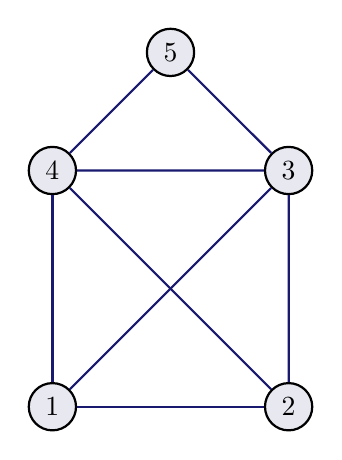
\begin{tikzpicture}[scale=1.5, thick,
  node/.style={circle, draw, fill=MidnightBlue!10, inner sep=0pt, minimum size=6mm}]
  
  \node[node] (1) at (0,0) {$1$};
  \node[node] (2) at (2,0) {$2$};
  \node[node] (3) at (2,2) {$3$};
  \node[node] (4) at (0,2) {$4$};
  \node[node] (5) at (1,3) {$5$};
  
  % Kanten
  \draw[MidnightBlue] (1) -- (2);
  \draw[MidnightBlue] (2) -- (3);
  \draw[MidnightBlue] (3) -- (4);
  \draw[MidnightBlue] (4) -- (1);
  \draw[MidnightBlue] (1) -- (3);
  \draw[MidnightBlue] (2) -- (4);
  \draw[MidnightBlue] (4) -- (5);
  \draw[MidnightBlue] (3) -- (5);
  
\end{tikzpicture}
\end{center}

\begin{explanation-of-steps}[Eulerweg im Haus vom Nikolaus]
Das Haus vom Nikolaus besitzt genau zwei Knoten mit ungeradem Grad ($\deg(1)=3$ und $\deg(2)=3$), während alle anderen Knoten geraden Grad besitzen ($\deg(3)=4, \deg(4)=4, \deg(5)=2$).

Nach dem Satz von Euler-Hierholzer existiert daher ein offener Eulerweg (ein Kantenzug, der jede Kante genau einmal enthält), welcher zwingend an einem der ungeraden Knoten (z.\,B. $1$) beginnen und am anderen ungeraden Knoten ($2$) enden muss. Ein geschlossener Eulerweg (Eulertour) existiert hingegen nicht.
\end{explanation-of-steps}
\end{math-stroke}

\begin{spoken-clean}[00:13:02 - 00:13:36]
Machen wir das Ganze vielleicht etwas systematischer und definieren alles sauber. Ich habe einen Teil der heutigen Vorlesung als Beamer-Präsentation vorbereitet. Das mache ich normalerweise nicht, aber wenn man so viele Definitionen hat, die alle sehr einfach sind, ist es etwas mühsam und zeitaufwendig, sie alle an die Tafel zu schreiben. Schauen wir uns das also lieber auf dem Beamer an.

So, sehen Sie das gut so? Gut.
\end{spoken-clean}

\begin{meta-note}[Projizierter Inhalt: Grundbegriffe der Graphentheorie]
Der Dozent schaltet den Projektor ein und zeigt die Folie \textbf{\qt{Grundbegriffe der Graphentheorie}} mit der formalen Definition eines Graphen:
\begin{definition}[Graph]
Ein \newterm{Graph} ist eine Menge $V$, deren Elemente wir \newterm{Knoten} nennen, zusammen mit einer Teilmenge $E \subseteq V \times V$ (oder mehreren Teilmengen $E_0, \dots, E_k \subseteq V \times V$), den sogenannten \newterm{Kanten}. Wir schreiben $G = (V, E)$, respektive $G = (V, E_0, \dots, E_k)$.
\end{definition}
\end{meta-note}

\begin{spoken-clean}[00:13:36 - 00:16:52]
Was ist also ein Graph? Ein Graph ist einfach eine Menge $V$, deren Elemente wir Knoten nennen, zusammen mit einer Teilmenge des kartesischen Produkts von $V$ mit sich selbst. Betrachten wir zuerst einmal diese Definition: Das sind die sogenannten Kanten.

Wir haben also $V$, unsere Knoten (englisch: \emph{vertices}, deswegen $V$). Und nun betrachten wir $V \times V$, also die geordneten Paare von Knoten; das sind unsere Kanten. Wir können uns das so vorstellen: Nehmen wir zum Beispiel die Knoten $1, 2, 3, 4$. Wir können sagen, zwischen zwei Knoten ziehen wir eine Kante. Das ist dann die Kante, die durch $1$ und $4$ gegeben ist. Sie führt von $1$ nach $4$, wenn wir sagen, es ist die Kante $\langle 1, 4 \rangle$.

Hier könnte eine Kante von $4$ nach $3$ führen, eine von $3$ nach $2$ und so weiter. Nach dieser Definition können wir jedoch nicht zwei Kanten von $4$ nach $3$ haben, weil es nur ein geordnetes Paar $\langle 4, 3 \rangle$ gibt. Das ist ein wichtiger Punkt. So sieht also nach dieser Definition ein Graph aus: Wir haben Knoten und betrachten die Kanten, die zwischen diesen Knoten liegen.

Was wir aber auch machen können: Wir können sagen, es gibt mehrere dieser Teilmengen, etwa $E_0$ bis $E_k$ von $V \times V$. Dann schreiben wir $G$ als $V$ zusammen mit all diesen Kantenmengen. So können wir natürlich mehrere Kanten haben. Hier könnten wir zum Beispiel sagen: Wir haben $E_0$, das ist diese Kante hier, und dann noch $E_1$, das ist diese Kante hier. Dann haben wir maximal zwei Kanten zwischen zwei Knoten. So lässt sich das definieren. Das ist die Definition eines Graphen.
\end{spoken-clean}

\begin{math-stroke}[Formale Definition eines Graphen]
\begin{definition}[Graph]\label[definition]{def:graph}
Ein \newterm{Graph} ist ein Paar $G = (V, E)$ (oder allgemeiner $G = (V, E_0, \dots, E_k)$), wobei:
\begin{itemize}
    \item $V$ eine nichtleere Menge von \newterm{Knoten} (engl. \newterm{vertices}) ist.
    \item $E \subseteq V \times V$ eine Menge von geordneten Paaren ist, welche die \newterm{Kanten} (engl. \newterm{edges}) repräsentieren.
    \item Falls Mehrfachkanten erlaubt sind, betrachten wir mehrere disjunkte Kantenmengen $E_0, \dots, E_k \subseteq V \times V$.
\end{itemize}
\end{definition}
\end{math-stroke}

\begin{spoken-clean}[00:16:52 - 00:20:32]
Hier gibt es auch noch ein bisschen Terminologie: Wir sagen, zwei Knoten $x, y \in V$ heißen \newterm{adjazent}, falls das Paar $\langle x, y \rangle$ in $E$ enthalten ist. Sie liegen also nebeneinander --- ein bisschen snobistisch ausgedrückt.

Das Nächste ist vielleicht ein bisschen verwirrend, aber wir sagen: Falls $E$ symmetrisch ist --- man kann $E$ ja auch als Relationssymbol auffassen, also als Teilmenge von $V \times V$ ---, dann ist der Graph \newterm{ungerichtet}. Das heißt, falls $\langle x, y \rangle$ in $E$ ist, dann ist auch $\langle y, x \rangle$ in $E$. In diesem Fall identifizieren wir einfach $\langle x, y \rangle$ mit $\langle y, x \rangle$ und schreiben das als ungerichtete Menge $\{x, y\}$, die in $E$ liegt.

Ein ungerichteter Graph ist eigentlich wie ein gerichteter Graph, bei dem man die Richtungen nicht unterscheidet. Lassen Sie sich von dieser Unterscheidung nicht zu stark verwirren; sie dient einfach der Einfachheit. Beim Königsberger Brückenproblem darf man auf den Brücken natürlich in beide Richtungen laufen. Man kann sowohl von hier nach dort als auch umgekehrt gehen. Ganz korrekt müsste man also sagen: Wir haben zwei Kanten, eine für jede Richtung. Das wäre wie eine Brücke mit Gegenverkehr.

Man kann aber auch sagen: Anstatt alle Kanten doppelt zu zeichnen, was etwas mühsam ist, zeichnen wir sie nur einfach ein und sagen, man darf in beide Richtungen laufen. Das Königsberger Brückenproblem wäre also ein Beispiel für einen ungerichteten Graphen.

Machen wir das noch einmal sauber: Beim Königsberger Graphen hätten wir die Knoten $1, 2, 3, 4$. Unsere Kanten wären hier ungerichtet, zum Beispiel $\{1, 4\}$. Dann hätten wir noch $\{3, 4\}$, $\{2, 3\}$ und $\{1, 2\}$. Und dann gäbe es vielleicht noch eine Menge $E_1$, die nochmals $\{3, 4\}$ und $\{2, 3\}$ enthält. Das wäre die formale Definition für diesen Fall.
\end{spoken-clean}

\begin{student-interaction}[Studentenfrage]
Ich habe eine kurze Frage: Macht das nicht eigentlich Eulers Argument kaputt? Weil man jetzt, wenn man einen ungerichteten Weg hin und zurück laufen kann... man muss ja irgendwie codieren, dass man jede Brücke nur einmal verwenden darf.
\end{student-interaction}

\begin{spoken-clean}[00:20:32 - 00:21:11]
Nur einmal, genau.
\end{spoken-clean}

\begin{student-interaction}[Studentenfrage continued]
Ja, wie sehe ich das? Für mich sieht es so aus, als hätte man einfach eine Brücke hin und eine Brücke zurück.
\end{student-interaction}

\begin{spoken-clean}[00:21:11 - 00:22:54]
Nein, hier haben wir jede Brücke nur noch einmal. Ein ungerichtetes Edge besteht zwar eigentlich aus zwei Tupeln, aber wir sagen: Wenn es ungerichtet ist, dann identifizieren wir die beiden und haben nur noch ein Objekt.

Ah, ich sehe gerade, wir haben da auch eine Kante vergessen, oder? $\{1, 2\}$ und $\{1, 3\}$ haben wir noch vergessen. Okay, dieser hier ist nicht derselbe wie jener dort. So viel zur Definition. Es ist ein bisschen mühsam, wenn man eine Definition nur als Definition sieht, aber es ist genau das, was Sie sich intuitiv unter einem Graphen vorstellen; es ist nicht so kompliziert.
\end{spoken-clean}

\begin{math-stroke}[Ungerichtete Graphen und Adjazenz]
\begin{definition}[Adjazenz]\label[definition]{def:adjazenz}
Zwei Knoten $x, y \in V$ heißen \newterm{adjazent} (benachbart), falls $\langle x, y \rangle \in E$ (bei gerichteten Graphen) bzw. $\{x, y\} \in E$ (bei ungerichteten Graphen).
\end{definition}

\begin{definition}[Ungerichteter Graph]\label[definition]{def:ungerichteter-graph}
Ein Graph $G = (V, E)$ heißt \newterm{ungerichtet}, falls die Relation $E \subseteq V \times V$ symmetrisch ist:
\[
\forall x, y \in V \colon \langle x, y \rangle \in E \iff \langle y, x \rangle \in E.
\]
In diesem Fall identifizieren wir die geordneten Paare $\langle x, y \rangle$ und $\langle y, x \rangle$ und schreiben sie als ungeordnete Paare (Mengen):
\[
\{x, y\} \in E.
\]
\end{definition}
\end{math-stroke}

\begin{spoken-clean}[00:22:54 - 00:25:30]
Wir sagen, ein Graph ist \newterm{gerichtet} oder ein \newterm{Digraph}, falls er nicht ungerichtet ist. Okay. Wunderbar, an Definitionen muss man sich ein bisschen gewöhnen.

Oft sagt man anstatt \qt{gerichtet} auch \qt{Digraph} --- weshalb Digraph? Eben weil es zwei verschiedene Richtungen gibt. Es hängt sehr stark vom Gebiet ab, in dem Sie arbeiten; ich würde sagen, man verwendet fast öfter ungerichtete Graphen als gerichtete.

Eine Kante der Form $\langle x, x \rangle$ heißt \newterm{Schlinge}. Es spricht nichts dagegen, so etwas zu haben. Das ist dann einfach eine solche Kante. Wenn es ein gerichteter Graph ist, würde man das einfach als $\langle x, x \rangle$ bezeichnen. Das ist natürlich dasselbe wie $\{x\}$. Eine Schlinge in einem gerichteten Graphen würde man so bezeichnen.

Hier müssen wir aufpassen: Eine Schlinge hat keine Richtung; man kann sie sich so oder so vorstellen, es bleibt $\langle x, x \rangle$. Ein Graph $G$ heißt \newterm{schlingenfrei}, falls er keine Schlingen hat.

Falls wir einen Graphen mit mehreren Kanten zwischen zwei Knoten haben --- wie beim Königsberger Graphen ---, dann nennen wir diese \newterm{Mehrfachkanten}. Hier gibt es zum Beispiel zwei Kanten zwischen zwei Knoten. Den Begriff braucht man aber vor allem, um das Gegenteil zu definieren: Ein Graph ohne Schlingen und ohne Mehrfachkanten heißt \newterm{schlicht}. Ein schlichter Graph ist also einfach ein Graph, der beides nicht hat.
\end{spoken-clean}

\begin{math-stroke}[Schlingen, Mehrfachkanten und schlichte Graphen]
\begin{definition}[Schlinge]\label[definition]{def:schlinge}
Eine Kante der Form $\langle x, x \rangle$ (bzw. $\{x, x\} = \{x\}$) heißt \newterm{Schlinge} (engl. \newterm{loop}).
\end{definition}

\begin{definition}[Mehrfachkanten]\label[definition]{def:mehrfachkanten}
Existieren zwischen zwei Knoten $x, y \in V$ mehr als eine Kante, so sprechen wir von \newterm{Mehrfachkanten} (engl. \newterm{multiple edges}). Ein solcher Graph wird auch als \newterm{Multigraph} bezeichnet.
\end{definition}

\begin{definition}[Schlichter Graph]\label[definition]{def:schlichter-graph}
Ein Graph $G = (V, E)$ heißt \newterm{schlicht} (oder \newterm{einfach}, engl. \newterm{simple graph}), falls er weder Schlingen noch Mehrfachkanten besitzt.
\end{definition}
\end{math-stroke}

\begin{spoken-clean}[00:25:30 - 00:28:30]
Schauen wir uns noch ein paar Beispiele an --- oder machen wir direkt weiter. Ich glaube, zu den Beispielen muss man nicht mehr viel sagen, das ist klar: Dieser Graph hier ist schlicht, jener dort ist wegen der Mehrfachkante nicht schlicht. Dieser hier ist wieder schlicht, aber der dort wegen der Schlinge nicht.

Die nächste Definition ist etwas ganz Nettes: Sei $G = (V, E)$ ein \newterm{endlicher Graph}. Ein endlicher Graph ist es dann, wenn es nur endlich viele Knoten gibt. Wenn es nur endlich viele Knoten gibt, dann gibt es auch nur endlich viele Kanten.

Einem solchen Graphen können wir eine Matrix zuordnen, die \newterm{Adjazenzmatrix}. Wir bezeichnen sie als $A(G)$ und schreiben ihre Einträge als $a_{ij}$. Dazu müssen wir $V$ zuerst durchnummerieren: $V = \{v_1, \dots, v_n\}$. Wir sagen nun: $a_{ij}$ ist $1$, falls es eine Kante von $v_i$ nach $v_j$ gibt, und $0$ sonst.
\end{spoken-clean}

\begin{didactic-insight}[Die Brücke zur Linearen Algebra: Warum Matrizen in der Graphentheorie?]
Die Einführung der Adjazenzmatrix ist weit mehr als eine bloße tabellarische Auflistung von Kanten. Sie schlägt eine fundamentale Brücke zur Linearen Algebra:
\begin{itemize}
    \item \textbf{Pfadzählung:} Ein zentrales Resultat besagt, dass der Eintrag $(i,j)$ der $k$-ten Potenz der Adjazenzmatrix, also $A(G)^k$, exakt der Anzahl aller gerichteten Kantenfolgen der Länge $k$ vom Knoten $v_i$ zum Knoten $v_j$ entspricht.
    \item \textbf{Spektrale Graphentheorie:} Die Eigenwerte der Adjazenzmatrix (das sogenannte Spektrum des Graphen) kodieren tiefgreifende strukturelle Eigenschaften des Graphen, wie etwa seine Konnektivität, chromatische Zahl oder ob er bipartit ist.
\end{itemize}
\end{didactic-insight}

\begin{spoken-clean}[00:28:30 - 00:31:12]
Ein Graph mit nur einer Kanten relation hat also eine Adjazenzmatrix, in der es nur $1$ und $0$ gibt, je nachdem, ob die Knoten verbunden sind oder nicht.

Machen wir ein Beispiel: Wir haben den Graphen mit den Knoten $1, 2, 3, 4$ und Kanten von $1$ nach $2$, von $2$ nach $3$, von $3$ nach $4$ und von $4$ nach $1$. Was wäre die Adjazenzmatrix dieses Graphen? Von $1$ nach $1$ gibt es nichts. Von $1$ nach $2$ gibt es eine Kante, sonst nichts. Von $2$ gibt es nur eine Kante nach $3$. Von $3$ gibt es eine nach $4$, und von $4$ gibt es eine nach $1$.

Falls wir mehrere Kanten zwischen zwei Knoten haben, ist es analog: Wir zählen einfach, wie viele Kanten es dazwischen gibt. Falls wir $G$ als $(V, E_0, \dots, E_k)$ schreiben --- wir haben also verschiedene Kantenmengen, aber immer noch endlich viele ---, dann ist die Adjazenzmatrix $A(G)$ definiert als die Summe von $\ell = 0$ bis $k$ über $A(G_\ell)$. Der Eintrag $a_{ij}$ ist dann einfach die Anzahl der Kanten von $v_i$ nach $v_j$.
\end{spoken-clean}

\subsection{Die Adjazenzmatrix}§

\begin{math-stroke}[Beispiele für schlichte Graphen und Adjazenzmatrix]
\begin{center}
\begin{tabular}{c c c c}
    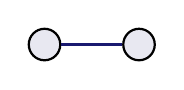
\begin{tikzpicture}[scale=0.8, thick]
        \node[circle, draw, fill=MidnightBlue!10, inner sep=0pt, minimum size=4mm] (A) at (0,0) {};
        \node[circle, draw, fill=MidnightBlue!10, inner sep=0pt, minimum size=4mm] (B) at (1.5,0) {};
        \draw[MidnightBlue] (A) -- (B);
    \end{tikzpicture} &
    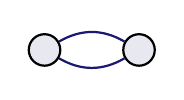
\begin{tikzpicture}[scale=0.8, thick]
        \node[circle, draw, fill=MidnightBlue!10, inner sep=0pt, minimum size=4mm] (A) at (0,0) {};
        \node[circle, draw, fill=MidnightBlue!10, inner sep=0pt, minimum size=4mm] (B) at (1.5,0) {};
        \draw[MidnightBlue] (A) to[bend left=30] (B);
        \draw[MidnightBlue] (A) to[bend right=30] (B);
    \end{tikzpicture} &
    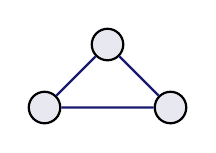
\begin{tikzpicture}[scale=0.8, thick]
        \node[circle, draw, fill=MidnightBlue!10, inner sep=0pt, minimum size=4mm] (A) at (0,0) {};
        \node[circle, draw, fill=MidnightBlue!10, inner sep=0pt, minimum size=4mm] (B) at (1,1) {};
        \node[circle, draw, fill=MidnightBlue!10, inner sep=0pt, minimum size=4mm] (C) at (2,0) {};
        \draw[MidnightBlue] (A) -- (B) -- (C) -- (A);
    \end{tikzpicture} &
    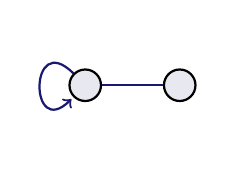
\begin{tikzpicture}[scale=0.8, thick]
        \node[circle, draw, fill=MidnightBlue!10, inner sep=0pt, minimum size=4mm] (A) at (0,0) {};
        \node[circle, draw, fill=MidnightBlue!10, inner sep=0pt, minimum size=4mm] (B) at (1.5,0) {};
        \draw[MidnightBlue] (A) -- (B);
        \path (A) edge[out=135, in=225, distance=1cm, loop, MidnightBlue] (A);
    \end{tikzpicture} \\
    \text{schlicht} & \text{nicht schlicht (Mehrfachkante)} & \text{schlicht} & \text{nicht schlicht (Schlinge)}
\end{tabular}
\end{center}


\begin{definition}[Adjazenzmatrix]\label[definition]{def:adjazenzmatrix}
Sei $G = (V, E)$ ein endlicher Graph mit durchnummerierten Knoten $V = \{v_1, \dots, v_n\}$. Die \newterm{Adjazenzmatrix} $A(G) = (a_{ij})_{1 \le i, j \le n}$ ist eine $n \times n$-Matrix definiert durch:
\[
a_{ij} := \begin{cases}
1 & \text{falls } \langle v_i, v_j \rangle \in E \text{ (bzw. } \{v_i, v_j\} \in E\text{)}, \\
0 & \text{sonst.}
\end{cases}
\]
Für einen Multigraphen $G = (V, E_0, \dots, E_k)$ ist $a_{ij} = \sum_{\ell=0}^k a_{ij}^{(\ell)}$ die Anzahl der Kanten von $v_i$ nach $v_j$:
\[
A(G) := \sum_{\ell=0}^k A(G_\ell).
\]
\end{definition}

\textbf{Beispiel für einen gerichteten Graphen und seine Adjazenzmatrix:}
\begin{center}
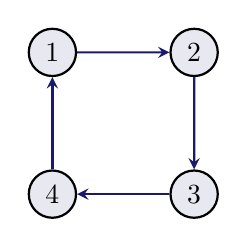
\begin{tikzpicture}[scale=1.2, ->, >=stealth, thick,
  node/.style={circle, draw, fill=MidnightBlue!10, inner sep=0pt, minimum size=6mm}]
  
  \node[node] (n1) at (0, 1.5) {$1$};
  \node[node] (n2) at (1.5, 1.5) {$2$};
  \node[node] (n3) at (1.5, 0) {$3$};
  \node[node] (n4) at (0, 0) {$4$};
  
  \path
    (n1) edge[MidnightBlue] (n2)
    (n2) edge[MidnightBlue] (n3)
    (n3) edge[MidnightBlue] (n4)
    (n4) edge[MidnightBlue] (n1);
\end{tikzpicture}
\end{center}
Die zugehörige Adjazenzmatrix lautet:
\[
A(G) = \begin{pmatrix}
0 & 1 & 0 & 0 \\
0 & 0 & 1 & 0 \\
0 & 0 & 0 & 1 \\
1 & 0 & 0 & 0
\end{pmatrix}
\]
\end{math-stroke}

\begin{spoken-clean}[00:31:12 - 00:32:57]
Falls wir mehrere Kanten zwischen zwei Knoten haben, ist es analog: Wir zählen einfach, wie viele Kanten es dazwischen gibt.

Falls wir $G$ als $(V, E_1, \dots, E_k)$ schreiben --- wir haben also verschiedene Kantenmengen, aber immer noch endlich viele ---, dann ist die Adjazenzmatrix $A(G)$ definiert als die Summe von $\ell = 1$ bis $k$ über $A(G_\ell)$. Der Eintrag $a_{ij}$ ist dann einfach die Anzahl der Kanten von $v_i$ nach $v_j$.
\end{spoken-clean}

\begin{math-stroke}[Adjazenzmatrix für Multigraphen]
Falls $G = (V, E_1, \dots, E_k)$ ein Multigraph mit endlich vielen Kantenmengen ist, definieren wir für jede Kantenmenge $E_\ell$ den Teilgraphen $G_\ell = (V, E_\ell)$. Die Adjazenzmatrix $A(G)$ ist dann die Summe der einzelnen Adjazenzmatrizen:
\begin{equation}
A(G) := \sum_{\ell=1}^k A(G_\ell)
\end{equation}
Der Eintrag $a_{ij}$ entspricht somit genau der Anzahl der Kanten, die vom Knoten $v_i$ zum Knoten $v_j$ führen.
\end{math-stroke}

\begin{spoken-clean}[00:32:57 - 00:34:42]
Schauen wir uns noch ein etwas komplizierteres Beispiel an; das steht auch im Skript. Wenn wir diesen Graphen hier betrachten: Von $1$ nach $1$ gibt es keine Kanten, dort steht also eine $0$. Von $1$ nach $2$ gibt es eine. Von $1$ nach $3$ gibt es keine, ebenso wenig nach $4$. Es gibt aber noch eine nach $5$ und eine nach $6$.

Von $2$ nach $1$ gibt es eine. Von $2$ nach $2$ gibt es keine, ebenso wenig nach $3$ oder $4$. Von $2$ nach $5$ gibt es eine, nach $6$ keine. Von $3$ nach $1$ gibt es keine, nach $2$ gibt es eine. Von $3$ nach $3$ gibt es eine Schlinge, und von $3$ nach $4$ gibt es zwei Kanten. Und so weiter. Das müssen wir jetzt nicht alles aufschreiben.
\end{spoken-clean}

\begin{math-stroke}[Komplexeres Beispiel eines gerichteten Multigraphen]
Wir betrachten den Graphen $G$ mit sechs Knoten $V = \{1, 2, 3, 4, 5, 6\}$, wie er auf der Folie projiziert wird:

\begin{center}
\begin{tikzpicture}[scale=1.5, ->, >=stealth, thick,
  node/.style={circle, draw, fill=MidnightBlue!10, inner sep=0pt, minimum size=7mm}]
  \begin{ai-tikz-planner-invisible-content}
  % 1. Background: Sechs Knoten kreisförmig angeordnet.
  % 2. Midground: Kanten mit Pfeilen, inklusive einer Schlinge an Knoten 3 und Doppelbindung zwischen 3 und 4.
  \end{ai-tikz-planner-invisible-content}
  \node[node] (n1) at (0, 2) {$1$};
  \node[node] (n2) at (2, 2) {$2$};
  \node[node] (n3) at (3, 1) {$3$};
  \node[node] (n4) at (2, 0) {$4$};
  \node[node] (n5) at (0, 0) {$5$};
  \node[node] (n6) at (-1, 1) {$6$};
  
  \path
    (n1) edge[bend left=15, MidnightBlue] (n2)
    (n2) edge[bend left=15, MidnightBlue] (n1)
    (n1) edge[MidnightBlue] (n5)
    (n6) edge[MidnightBlue] (n1)
    (n6) edge[MidnightBlue] (n5)
    (n6) edge[MidnightBlue] (n2)
    (n2) edge[MidnightBlue] (n5)
    (n3) edge[MidnightBlue] (n2)
    (n3) edge[out=45, in=-45, distance=0.8cm, loop, MidnightBlue] (n3)
    (n3) edge[bend left=15, MidnightBlue] (n4)
    (n3) edge[bend right=15, MidnightBlue] (n4)
    (n4) edge[MidnightBlue] (n3)
    (n4) edge[bend left=15, MidnightBlue] (n5)
    (n5) edge[bend left=15, MidnightBlue] (n4)
    (n5) edge[MidnightBlue] (n3);
\end{tikzpicture}
\end{center}

Die an der Tafel unvollständig skizzierte Adjazenzmatrix $A(G)$ lautet:
\[
A(G) = \begin{pmatrix}
0 & 1 & 0 & 0 & 1 & 1 \\
1 & 0 & 0 & 0 & 1 & 0 \\
0 & 1 & 1 & 2 & 0 & 0 \\
\vdots & \vdots & \vdots & \vdots & \vdots & \vdots
\end{pmatrix}
\]

\begin{explanation-of-steps}[Vollständige Adjazenzmatrix]
Unter Berücksichtigung aller Kanten des projizierten Graphen ergibt sich die vollständige Adjazenzmatrix:
\[
A(G) = \begin{pmatrix}
0 & 1 & 0 & 0 & 1 & 1 \\
1 & 0 & 0 & 0 & 1 & 0 \\
0 & 1 & 1 & 2 & 0 & 0 \\
0 & 0 & 1 & 0 & 1 & 0 \\
0 & 0 & 1 & 1 & 0 & 0 \\
1 & 1 & 0 & 0 & 1 & 0
\end{pmatrix}
\]
\end{explanation-of-steps}
\end{math-stroke}

\begin{spoken-clean}[00:34:42 - 00:35:22]
Ist das klar? Gut. Machen wir weiter mit ein paar Bemerkungen, die relativ einfach aus der Definition folgen. Wenn $A(G)$ die Adjazenzmatrix ist...
\end{spoken-clean}

\begin{math-stroke}[Eigenschaften der Adjazenzmatrix]
\begin{remark}[Eigenschaften der Adjazenzmatrix]\label[remark]{rem:adjazenzmatrix-eigenschaften}
Sei $G = (V, E)$ ein endlicher Graph und $A(G) = (a_{ij})$ seine Adjazenzmatrix.
\begin{enumerate}[label=\textbf{(\roman*)}]
    \item \textbf{Nichtnegativität:} Alle Einträge der Adjazenzmatrix sind nichtnegative ganze Zahlen:
    \[
    a_{ij} \ge 0 \quad \text{und} \quad a_{ij} \in \mathbb{N}_0 \quad (\text{bzw. } \omega).
    \]
    \item \textbf{Schlingenfreiheit:} Der Graph $G$ ist schlingenfrei genau dann, wenn alle Diagonalelemente der Adjazenzmatrix null sind:
    \[
    G \text{ ist schlingenfrei} \iff a_{ii} = 0 \quad \forall i \in \{1, \dots, n\}.
    \]
    Dies ist äquivalent dazu, dass die Spur der Matrix verschwindet:
    \[
    \operatorname{Sp}(A(G)) = \sum_{i=1}^n a_{ii} = 0.
    \]
\end{enumerate}
\end{remark}
\end{math-stroke}

\begin{spoken-clean}[00:35:22 - 00:37:30]
Wie sieht man an der Adjazenzmatrix, ob der Graph ungerichtet ist oder nicht? Noch eine weitere Bemerkung: Der Graph $G$ ist ungerichtet genau dann, wenn die Matrix symmetrisch ist. Das ist klar: Das ist der Fall, wenn für jede Kante $v_i \to v_j$ auch $v_j \to v_i$ eine Kante ist. Und das ist äquivalent dazu, dass die Matrix symmetrisch ist.
\end{spoken-clean}

\begin{spoken-clean}[00:37:30 - 00:39:52]
Das heißt, $G$ ist ungerichtet genau dann, wenn die Adjazenzmatrix symmetrisch ist. Man sieht also an der Symmetrie der Matrix direkt, ob der Graph ungerichtet ist oder nicht.
\end{spoken-clean}

\begin{math-stroke}[Symmetrie ungerichteter Graphen]
\begin{remark}[Symmetrie]\label[remark]{rem:symmetrie-adjazenz}
Ein Graph $G$ ist ungerichtet genau dann, wenn seine Adjazenzmatrix $A(G)$ symmetrisch ist:
\[
G \text{ ist ungerichtet} \iff A(G) = A(G)^T \iff a_{ij} = a_{ji} \quad \forall i, j \in \{1, \dots, n\}.
\]
\end{remark}
\end{math-stroke}

\section{Knotengrad (Degree)}
\subsection{Knotengrad in gerichteten Graphen (Digraphen)}

\begin{spoken-clean}[00:39:52 - 00:42:57]
Machen wir noch ein paar weitere Definitionen an der Tafel, und danach machen wir eine Pause.

Sei $G = (V, E)$ ein Digraph, also ein gerichteter Graph. Für einen Knoten $x \in V$ definieren wir zuerst einmal $\Gamma^+(x)$. Das definieren wir als die Menge aller Knoten $y \in V$, sodass $\langle x, y \rangle$ eine Kante ist. Das sind quasi alle... wenn Sie hier $x$ haben, dann schreiben wir alle $y$ auf, sodass es eine Kante von $x$ nach $y$ gibt. Das ist diese Menge hier.

Analog ist $\Gamma^-(x)$ die Menge aller $y \in V$, sodass $\langle y, x \rangle$ eine Kante ist. Das sind also alle $y$, von denen eine Kante nach $x$ führt.

Gut, und dann definieren wir den \newterm{positiven Halbgrad} $\deg^+(x)$ als die Kardinalität von $\Gamma^+(x)$. Und den \newterm{negativen Halbgrad} $\deg^-(x)$ als die Kardinalität von $\Gamma^-(x)$.
\end{spoken-clean}

\begin{spoken-clean}[00:42:57 - 00:45:02]
Und was ist dann der \newterm{Grad} von $x$? Den definieren wir als die Summe vom positiven und dem negativen Halbgrad. Das ist also die Anzahl der Kanten, die mit $x$ verbunden sind. Schauen wir uns dazu ein kurzes Beispiel an, bevor wir Pause machen: Wenn $x$ eine Schlinge hat, was ist dann der Grad von $x$?

Zwei, genau! Weil wir hier eine Kante haben, die einmal hinausgeht und einmal hineinkommt; sie wird also zweimal gezählt. Das macht Sinn und ist genau das, was wir haben wollen.
\end{spoken-clean}

\begin{math-stroke}[Halbgrade und Grad in Digraphen]
\begin{definition}[Halbgrade und Grad]\label[definition]{def:halbgrade-grad}
Sei $G = (V, E)$ ein Digraph. Für einen Knoten $v \in V$ definieren wir:
\begin{itemize}
    \item \textbf{Ausgangsnachbarschaft:} $\Gamma^+(v) := \{ w \in V \mid \langle v, w \rangle \in E \}$
    \item \textbf{Eingangsnachbarschaft:} $\Gamma^-(v) := \{ u \in V \mid \langle u, v \rangle \in E \}$
    \item \textbf{Ausgangsgrad (positiver Halbgrad):} $\deg^+(v) := |\Gamma^+(v)|$
    \item \textbf{Eingangsgrad (negativer Halbgrad):} $\deg^-(v) := |\Gamma^-(v)|$
    \item \textbf{Grad:} $\deg(v) := \deg^+(v) + \deg^-(v)$
\end{itemize}
\end{definition}

\begin{center}
\begin{tikzpicture}[scale=1.2, ->, >=stealth, thick,
  node/.style={circle, draw, fill=MidnightBlue!10, inner sep=0pt, minimum size=6mm}]
  \begin{ai-tikz-planner-invisible-content}
  % 1. Background: Zentraler Knoten x.
  % 2. Midground: Ausgehende Kanten zu y1, y2, y3.
  \end{ai-tikz-planner-invisible-content}
  \node[node] (x) at (0,0) {$x$};
  \node[node] (y1) at (1.5, 0.8) {$y_1$};
  \node[node] (y2) at (1.8, 0) {$y_2$};
  \node[node] (y3) at (1.5, -0.8) {$y_3$};
  
  \draw[MidnightBlue] (x) -- (y1);
  \draw[MidnightBlue] (x) -- (y2);
  \draw[MidnightBlue] (x) -- (y3);
  
  \node[right=0.2cm of y2, MidnightBlue] {$\Gamma^+(x) = \{y_1, y_2, y_3\}$};
\end{tikzpicture}
\end{center}
\end{math-stroke}

\begin{lecture-break}[Pause]
Der Dozent kündigt eine kurze Pause an. Die Vorlesung wird nach der Pause mit der Definition des Knotengrads für ungerichtete Graphen fortgesetzt.
\end{lecture-break}

\subsection{Knotengrad in ungerichteten Graphen}

\begin{spoken-clean}[00:45:02 - 00:47:12]
Wir machen langsam weiter. Wir hatten vor der Pause die Definition des Grades für gerichtete Graphen gesehen. Wenn unser Graph ungerichtet ist, dann definieren wir $\Gamma(x)$ --- dort gibt es kein $\Gamma^+$ und $\Gamma^-$ mehr --- einfach als die Menge aller $y \in V$, sodass $\{x, y\} \in E$ ist.

In diesem Fall definieren wir den Grad von $x$ so, dass wir das Richtige erhalten: Uns interessiert die Richtung nicht mehr, weil sie dieselbe ist. Wenn wir so einen Graphen haben --- ungerichteter Graph ---, wollen wir einfach, dass dieser Knoten hier Grad $4$ hat. Das ist im Prinzip einfach die Anzahl der $y$, sodass $\{x, y\}$ eine Kante ist, also die Anzahl der Kanten, die von hier ausgehen. Das definieren wir als die Kardinalität von $\Gamma(x)$.
\end{spoken-clean}

\begin{spoken-clean}[00:47:12 - 00:49:12]
Was wir jetzt noch für ein Problem haben, ist die Schlinge. Wenn wir so etwas haben, wird das im Moment nur einmal gezählt. Wir hätten aber gerne, dass das auch im ungerichteten Fall Grad $2$ hat.

Deswegen müssen wir, wenn es eine Schlinge gibt, diese noch einmal dazuzählen. Das ist diese technische Definition im Skript: die Menge aller $x \in V$, sodass $\{x\}$ eine Kante ist. Da $x$ gegeben ist, besteht diese Menge entweder aus $x$ oder sie ist leer. Das heißt, wir müssen entweder $0$ oder $1$ zusätzlich addieren.

Das ist die Definition des Grades für ungerichtete Graphen. Sowohl für gerichtete als auch für ungerichtete Graphen gilt: Falls unser Graph von der Form $G = (V, E_0, \dots, E_k)$ ist, kann man das wieder genau gleich definieren, indem man die Summe über alle Teilgraphen nimmt.
\end{spoken-clean}

\begin{math-stroke}[Grad in ungerichteten Graphen und Multigraphen]
\begin{definition}[Ungerichteter Knotengrad]\label[definition]{def:ungerichteter-grad}
Sei $G = (V, E)$ ein ungerichteter Graph. Für einen Knoten $x \in V$ definieren wir:
\begin{itemize}
    \item \textbf{Nachbarschaft:} $\Gamma(x) := \{ y \in V \mid \{x, y\} \in E \}$
    \item \textbf{Grad:} 
    \begin{equation}
    \deg(x) := |\Gamma(x)| + \left| \{ y \in V \mid \{y\} \in E \land y = x \} \right|
    \end{equation}
\end{itemize}
\end{definition}

\begin{explanation-of-steps}[Kompensation für Schlingen]
Die Addition des Terms $\left| \{ y \in V \mid \{y\} \in E \land y = x \} \right|$ stellt sicher, dass eine Schlinge $\{x\}$ am Knoten $x$ doppelt zum Grad beiträgt (einmal als ausgehende und einmal als eingehende Kante), was der anschaulichen geometrischen Vorstellung entspricht.
\end{explanation-of-steps}

\textbf{Erweiterung auf Multigraphen:}
Für einen Multigraphen $G = (V, E_0, \dots, E_k)$ definieren wir den Grad analog als Summe der Grade in den einzelnen Kantenrelationen:
\begin{align}
    \deg_G(x) &:= \sum_{\ell=0}^k \deg_{G_\ell}(x) \\
    \deg^+_G(x) &:= \sum_{\ell=0}^k \deg^+_{G_\ell}(x) \\
    \deg^-_G(x) &:= \sum_{\ell=0}^k \deg^-_G(x)
\end{align}
\end{math-stroke}

\section{Spezielle Graphenklassen}
\subsection{Reguläre Graphen}

\begin{spoken-clean}[00:49:12 - 00:52:42]
Das ist einfach so definiert, damit es das ergibt, was man möchte. Machen wir die folgende Definition: Ein ungerichteter Graph heißt \newterm{regulär vom Grad $r$}, falls der Grad von $x$ gleich $r$ ist für alle $x \in V$. Das heißt also: Falls alle Knoten denselben Grad haben, ist der Graph regulär.

Zum Beispiel ist dieser Graph hier regulär vom Grad $2$. Oder wir können uns einen unendlichen Graphen anschauen: Wenn man zum Beispiel hier beginnt und von einem Knoten drei Kanten weggehen lässt, und dann gehen von den nächsten Knoten jeweils wieder zwei weg... das geht dann immer so weiter. Das ist ein sogenannter \newterm{Baum}, der ist auch regulär vom Grad $3$.
\end{spoken-clean}

\begin{math-stroke}[Reguläre Graphen]
\begin{definition}[Regulärer Graph]\label[definition]{def:regulaerer-graph}
Ein ungerichteter Graph $G = (V, E)$ heißt \newterm{regulär vom Grad $r$} (oder kurz \newterm{$r$-regulär}), falls alle seine Knoten denselben Grad $r$ besitzen:
\[
\forall x \in V \colon \deg(x) = r.
\]
\end{definition}

\textbf{Beispiele regulärer Graphen:}
\begin{center}
\begin{tabular}{c c}
    \begin{tikzpicture}[scale=1.2, thick,
      node/.style={circle, draw, fill=MidnightBlue!10, inner sep=0pt, minimum size=6mm}]
      \begin{ai-tikz-planner-invisible-content}
      % 1. Background: Vier Knoten als Quadrat.
      % 2. Midground: Kanten im Kreis (2-regulär).
      \end{ai-tikz-planner-invisible-content}
      \node[node] (1) at (0,1.5) {$1$};
      \node[node] (2) at (1.5,1.5) {$2$};
      \node[node] (3) at (1.5,0) {$3$};
      \node[node] (4) at (0,0) {$4$};
      \draw[MidnightBlue] (1) -- (2) -- (3) -- (4) -- (1);
    \end{tikzpicture} &
    \begin{tikzpicture}[scale=1.0, thick,
      node/.style={circle, draw, fill=MidnightBlue!10, inner sep=0pt, minimum size=4mm}]
      \begin{ai-tikz-planner-invisible-content}
      % 1. Background: Unendlicher Baum regulär vom Grad 3 (Cayley-Baum).
      \end{ai-tikz-planner-invisible-content}
      \node[node] (c) at (0,0) {};
      \node[node] (n1) at (90:0.8) {};
      \node[node] (n2) at (210:0.8) {};
      \node[node] (n3) at (330:0.8) {};
      \draw[MidnightBlue] (c) -- (n1) (c) -- (n2) (c) -- (n3);
      \node[node] (n11) at (60:1.5) {};
      \node[node] (n12) at (120:1.5) {};
      \node[node] (n21) at (180:1.5) {};
      \node[node] (n22) at (240:1.5) {};
      \node[node] (n31) at (300:1.5) {};
      \node[node] (n32) at (0:1.5) {};
      \draw[MidnightBlue] (n1) -- (n11) (n1) -- (n12);
      \draw[MidnightBlue] (n2) -- (n21) (n2) -- (n22);
      \draw[MidnightBlue] (n3) -- (n31) (n3) -- (n32);
    \end{tikzpicture} \\
    \text{2-regulärer Graph $C_4$} & \text{3-regulärer unendlicher Baum}
        \end{tabular}
        \end{center}
\end{math-stroke}

\subsection{Vollständige Graphen}

\begin{spoken-clean}[00:52:42 - 00:56:27]
Ein ungerichteter Graph $G = (V, E)$ heißt \newterm{vollständig}, falls für alle $x, y \in V$ gilt: $x \neq y \implies \{x, y\} \in E$. Das heißt, falls alle Knoten miteinander verbunden sind, ist der Graph vollständig.

Wenn wir eine Menge von Knoten gegeben haben, gibt es nur einen vollständigen Graphen, weil wir alle möglichen Kanten dazunehmen müssen, die keine Schlingen sind. Wir führen eine Notation ein: Wir sagen, $K_n$ ist der vollständige schlichte Graph mit $n$ Knoten. Machen wir das doch so wie im Skript. Für Lorenz Halbeisen ist \qt{vollständig} nicht unbedingt schlicht, aber wir legen fest, dass $K_n$ der vollständige schlichte Graph mit $n$ Knoten ist.

Zum Beispiel wäre das hier $K_3$: Er hat drei Knoten und ist vollständig. $K_4$ können wir auch zeichnen: Wir haben vier Knoten und müssen jeden mit jedem verbinden. Also verbinden wir diese hier, dann den dort mit jenem, mit diesem und mit dem anderen. Und fertig. Das ist $K_4$. Es gibt auch $K_5$, den zu zeichnen wird etwas schwierig, ohne dass sich Kanten überschneiden, aber man kann es machen.

Noch eine Bemerkung: Ich behaupte, $K_n$ ist immer regulär. Von welchem Grad? Genau, $n-1$. Da der $K_n$ schlicht ist, gibt es keine Schlingen. Von jedem Punkt aus muss eine Kante zu jedem anderen Knoten gehen. Das sind also genau $n-1$ Kanten, die von jedem Knoten ausgehen.
\end{spoken-clean}

\begin{math-stroke}[Das Konzept des vollständigen Graphen]
\begin{definition}[Vollständiger Graph]\label[definition]{def:vollstaendiger-graph}
Ein ungerichteter, schlichter Graph $G = (V, E)$ heißt \newterm{vollständig}, falls alle Paare verschiedener Knoten durch eine Kante verbunden sind:
\[
\forall x, y \in V \colon x \neq y \implies \{x, y\} \in E.
\]
Wir bezeichnen den vollständigen schlichten Graphen mit $n$ Knoten als $K_n$.
\end{definition}

\textbf{Beispiele vollständiger Graphen:}
\begin{center}
\begin{tabular}{c c}
    \begin{tikzpicture}[scale=1.2, thick,
      node/.style={circle, draw, fill=MidnightBlue!10, inner sep=0pt, minimum size=6mm}]
      \begin{ai-tikz-planner-invisible-content}
      % 1. Background: Drei Knoten als Dreieck (K_3).
      \end{ai-tikz-planner-invisible-content}
      \node[node] (1) at (90:0.8) {$1$};
      \node[node] (2) at (210:0.8) {$2$};
      \node[node] (3) at (330:0.8) {$3$};
      \draw[MidnightBlue] (1) -- (2) -- (3) -- (1);
    \end{tikzpicture} &
    \begin{tikzpicture}[scale=1.2, thick,
      node/.style={circle, draw, fill=MidnightBlue!10, inner sep=0pt, minimum size=6mm}]
      \begin{ai-tikz-planner-invisible-content}
      % 1. Background: Vier Knoten als Quadrat mit Diagonalen (K_4).
      \end{ai-tikz-planner-invisible-content}
      \node[node] (1) at (45:1.0) {$1$};
      \node[node] (2) at (135:1.0) {$2$};
      \node[node] (3) at (225:1.0) {$3$};
      \node[node] (4) at (315:1.0) {$4$};
      \draw[MidnightBlue] (1) -- (2) -- (3) -- (4) -- (1);
      \draw[MidnightBlue] (1) -- (3);
      \draw[MidnightBlue] (2) -- (4);
    \end{tikzpicture} \\
    \text{Vollständiger Graph $K_3$} & \text{Vollständiger Graph $K_4$}
\end{tabular}
\end{center}

\begin{proposition}[Regularität vollständiger Graphen]\label[proposition]{prop:k_n-regulaer}
Der vollständige schlichte Graph $K_n$ ist regulär vom Grad $n-1$:
\[
\forall v \in V(K_n) \colon \deg(v) = n-1.
\]
\end{proposition}
\end{math-stroke}

\subsection{Teilgraphen (Subgraphen)}

\begin{spoken-clean}[00:56:27 - 00:58:25]
Heute haben wir viele Definitionen gesehen; das war etwas mühsam, mit all diesen neuen Konzepten, aber nichts davon ist schwierig, es ist einfach viel. Versuchen Sie doch, die Übungen zu machen; das sind ganz nette Knobelaufgaben.

Wir kommen zur nächsten Definition: Wir nehmen an, dass wir Graphen $G = (V, E)$ und $G' = (V', E')$ haben, sodass $V' \subseteq V$ und $E' \subseteq E$ gilt. Dann ist $G'$ ein \newterm{Teilgraph} von $G$. Wir schreiben $G' \subseteq G$.

Das ist also klar: Wir nehmen eine Teilmenge von Knoten, und alle Kanten in unserem Graphen $G'$ müssen auch Kanten in $G$ sein. Das ist ein Teilgraph.
\end{spoken-clean}

\begin{math-stroke}[Teilgraphen]
\begin{definition}[Teilgraph]\label[definition]{def:teilgraph}
Seien $G = (V, E)$ und $G' = (V', E')$ zwei Graphen. $G'$ heißt ein \newterm{Teilgraph} (oder \newterm{Subgraph}) von $G$, falls gilt:
\[
V' \subseteq V \quad \text{und} \quad E' \subseteq E.
\]
Wir schreiben dafür $G' \subseteq G$.
\end{definition}
\end{math-stroke}

\begin{spoken-clean}[00:58:25 - 01:01:14]
Wenn wir nun einfach eine Menge von Knoten $U$ haben, können wir den größten Teilgraphen in $G$ betrachten, der nur diese Knoten hat. Das heißt, wir nehmen alle Kanten aus $G$ dazu, die Knoten in $U$ verbinden. Das ist der \newterm{von $U$ erzeugte Teilgraph}.

Gleichzeitig können wir das auch für Kanten definieren: Wenn $F$ eine Teilmenge der Kanten $E$ ist, dann definieren wir den \newterm{von $F$ erzeugten Teilgraph}. Das ist der Teilgraph mit den Knoten, die in diesen Kanten vorkommen. Das ist also die Vereinigung aller Knoten $x, y$ in $V$, sodass $\{x, y\}$ in $F$ liegt. Als Kanten nehmen wir natürlich genau die Kanten aus $F$.
\end{spoken-clean}

\begin{math-stroke}[Erzeugte Teilgraphen]
\begin{definition}[Knoteninduzierter Teilgraph]\label[definition]{def:knoteninduzierter-teilgraph}
Sei $G = (V, E)$ ein Graph und $U \subseteq V$ eine Teilmenge der Knoten. Der von $U$ \newterm{induzierte Teilgraph} (oder \newterm{erzeugte Teilgraph}) $G[U] = (U, E_U)$ hat die Knotenmenge $U$ und die Kantenmenge:
\[
E_U := \{ \{x, y\} \in E \mid x, y \in U \} \quad (\text{bzw. } \langle x, y \rangle \in E \text{ für Digraphen}).
\]
\end{definition}

\begin{definition}[Kanteninduzierter Teilgraph]\label[definition]{def:kanteninduzierter-teilgraph}
Sei $G = (V, E)$ ein Graph und $F \subseteq E$ eine Teilmenge der Kanten. Der von $F$ \newterm{erzeugte Teilgraph} $G[F] = (V_F, F)$ hat die Kantenmenge $F$ und die Knotenmenge $V_F$, welche aus allen Endknoten der Kanten in $F$ besteht:
\[
V_F := \bigcup_{\{x, y\} \in F} \{x, y\} \quad (\text{bzw. } \bigcup_{\langle x, y \rangle \in F} \{x, y\}).
\]
\end{definition}
\end{math-stroke}

\subsection{Pfeilzüge in gerichteten Graphen}

\begin{spoken-clean}[01:01:14 - 01:07:24]
Wir kommen nun zu den \newterm{Pfeilzügen}. Pfeilzüge beziehen sich auf Digraphen, da Pfeile eine Richtung haben. Wir sagen: Wenn wir einen Digraphen $(V, E)$ haben und $H$ eine nichtleere, endliche Kantenteilmenge ist, sodass $|H| = \ell$ gilt --- es gibt also genau $\ell$ Kanten in dieser Teilmenge --- und $H$ von der Form $\langle x_0, x_1 \rangle, \langle x_1, x_2 \rangle, \dots$ ist, wobei der Endpunkt einer Kante der Anfangspunkt der nächsten ist, dann heißt der durch $H$ erzeugte Teilgraph ein \newterm{Pfeilzug} von $x_0$ nach $x_\ell$ der Länge $\ell$.

Ich mache dazu ein Bild: Bei einem Pfeilzug beginnen wir bei $x_0$, gehen zu $x_1$, dann zu $x_2$, bis wir irgendwann bei $x_\ell$ ankommen. Dieser Teilgraph ist dann der Pfeilzug.

Hier muss man bemerken: In dieser Definition müssen diese Kanten alle verschieden sein, da die Kanten genau die Menge $H$ bilden; es müssen also $\ell$ verschiedene Kanten sein. Was jedoch nicht verlangt wird, ist, dass die Knoten verschieden sind. Man darf mehrmals über denselben Knoten gehen. Erlaubt ist zum Beispiel so etwas. Das ist okay, solange die Kanten verschieden sind.

Es gibt zwei verschiedene Arten von Pfeilzügen: Die einen sind \newterm{offene Pfeilzüge}, bei denen Anfangs- und Endpunkt verschieden sind, und die anderen sind \newterm{geschlossen}, falls man wieder zum Ursprung zurückkehrt, der Anfangspunkt also derselbe ist wie der Endpunkt.

Falls die Knoten $x_i$ paarweise verschieden sind, heißt das Ganze eine \newterm{Bahn}. Eine Bahn der Länge $\ell$ zwischen $x_0$ und $x_\ell$. Es macht Sinn, dass sie die Länge $\ell$ hat, weil $\ell$ Kanten vorkommen. Falls alle Knoten außer dem Anfangs- und Endpunkt verschieden sind, nennt man es einen \newterm{Wirbel}. Das ist wie ein Kreis, der eine Richtung hat.
\end{spoken-clean}

\begin{math-stroke}[Pfeilzüge in gerichteten Graphen]
\begin{definition}[Pfeilzug]\label[definition]{def:pfeilzug}
Sei $G = (V, E)$ ein Digraph und sei $H \subseteq E$ eine nichtleere, endliche Kantenteilmenge, sodass für ein $\ell \ge 1$ gilt: $|H| = \ell$ und
\[
H = \{ \langle x_0, x_1 \rangle, \langle x_1, x_2 \rangle, \dots, \langle x_{\ell-1}, x_\ell \rangle \}.
\]
Der durch $H$ erzeugte Teilgraph $G[H]$ heißt \newterm{Pfeilzug} von $x_0$ nach $x_\ell$ der Länge $\ell$.
\begin{itemize}
    \item Ein Pfeilzug heißt \newterm{offen}, falls $x_0 \neq x_\ell$.
    \item Ein Pfeilzug heißt \newterm{geschlossen}, falls $x_0 = x_\ell$.
\end{itemize}
\end{definition}

\begin{center}
\begin{tikzpicture}[scale=1.2, ->, >=stealth, thick,
  node/.style={circle, draw, fill=MidnightBlue!10, inner sep=0pt, minimum size=6mm}]
  \begin{ai-tikz-planner-invisible-content}
  % 1. Background: Pfad von x0 bis xl.
  \end{ai-tikz-planner-invisible-content}
  \node[node] (x0) at (0,0) {$x_0$};
  \node[node] (x1) at (1.5,0.5) {$x_1$};
  \node[node] (x2) at (3,0) {$x_2$};
  \node[node] (xl) at (4.5,0.5) {$x_\ell$};
  
  \path
    (x0) edge[MidnightBlue] (x1)
    (x1) edge[MidnightBlue] (x2)
    (x2) edge[dashed, MidnightBlue] (xl);
\end{tikzpicture}
\end{center}

\begin{definition}[Bahn und Wirbel]\label[definition]{def:bahn-wirbel}
Sei $G[H]$ ein Pfeilzug der Länge $\ell$ von $x_0$ nach $x_\ell$:
\begin{itemize}
    \item Falls die Knoten $x_0, \dots, x_\ell$ paarweise verschieden sind, so heißt $G[H]$ eine \newterm{Bahn} der Länge $\ell$ zwischen $x_0$ und $x_\ell$.
    \item Falls $x_0 = x_\ell$ und die Knoten $x_0, \dots, x_{\ell-1}$ paarweise verschieden sind, so heißt $G[H]$ ein \newterm{Wirbel} der Länge $\ell$.
\end{itemize}
\end{definition}
\end{math-stroke}

\subsection{Kantenzüge in ungerichteten Graphen}

\begin{spoken-clean}[01:07:24 - 01:10:00]
Dann gibt es \newterm{Kantenzüge}, und das ist genau dieselbe Definition, jetzt einfach für ungerichtete Graphen. Oh je, oh je --- das muss man fast korrigieren. Wenn wir mit ungerichteten Graphen arbeiten, heißt das Ganze Kantenzug anstatt Pfeilzug. Schreiben wir das auf.

Manchmal schleichen sich Tippfehler ein, die darf man nicht stehen lassen. Wenn wir also einen ungerichteten Graphen haben und eine nichtleere, endliche Kantenteilmenge $H$, sodass für ein $\ell \ge 1$ gilt: $|H| = \ell$ und $H = \{ \{x_0, x_1\}, \{x_1, x_2\}, \dots, \{x_{\ell-1}, x_\ell\} \}$. Dann heißt der durch $H$ erzeugte Teilgraph $G[H]$ ein \newterm{Kantenzug} von $x_0$ nach $x_\ell$ der Länge $\ell$.
\end{spoken-clean}

\begin{spoken-clean}[01:10:00 - 01:14:24]
Auch hier wieder: Ein Kantenzug heißt offen oder geschlossen. Und anstelle von \qt{Bahn} und \qt{Wirbel} sagen wir bei ungerichteten Graphen \newterm{Weg} oder \newterm{Kreis}. Das sind einfach zwei verschiedene Welten der Notation, aber für ungerichtete Graphen ist es genau dieselbe Definition. Das können wir noch kurz aufschreiben.
\end{spoken-clean}

\begin{math-stroke}[Kantenzüge in ungerichteten Graphen]
\begin{definition}[Kantenzug]\label[definition]{def:kantenzug}
Sei $G = (V, E)$ ein ungerichteter Graph und sei $H \subseteq E$ eine nichtleere, endliche Kantenteilmenge, sodass für ein $\ell \ge 1$ gilt: $|H| = \ell$ und
\[
H = \{ \{x_0, x_1\}, \{x_1, x_2\}, \dots, \{x_{\ell-1}, x_\ell\} \}.
\]
Der durch $H$ erzeugte Teilgraph $G[H]$ heißt \newterm{Kantenzug} von $x_0$ nach $x_\ell$ der Länge $\ell$.
\begin{itemize}
    \item Ein Kantenzug heißt \newterm{offen}, falls $x_0 \neq x_\ell$.
    \item Ein Kantenzug heißt \newterm{geschlossen}, falls $x_0 = x_\ell$.
\end{itemize}
\end{definition}

\begin{definition}[Weg und Kreis]\label[definition]{def:weg-kreis}
Sei $G[H]$ ein Kantenzug der Länge $\ell$ von $x_0$ nach $x_\ell$:
\begin{itemize}
    \item Falls die Knoten $x_0, \dots, x_\ell$ paarweise verschieden sind, so heißt $G[H]$ ein \newterm{Weg} der Länge $\ell$ zwischen $x_0$ und $x_\ell$.
    \item Falls $x_0 = x_\ell$ und die Knoten $x_0, \dots, x_{\ell-1}$ paarweise verschieden sind, so heißt $G[H]$ ein \newterm{Kreis} der Länge $\ell$.
\end{itemize}
\end{definition}

\textbf{Vergleich der Terminologie:}
\begin{center}
\begin{tabular}{l l}
    \toprule
    \textbf{Gerichtete Graphen (Digraphen)} & \textbf{Ungerichtete Graphen} \\
    \midrule
    Pfeilzug & Kantenzug \\
    Bahn & Weg \\
    Wirbel & Kreis \\
    \bottomrule
\end{tabular}
\end{center}
\end{math-stroke}

\section{Kombinatorische Eigenschaften und Pfadzählung}
\subsection{Pfadzählung mittels Adjazenzmatrix}

\begin{spoken-clean}[01:14:24 - 01:17:18]
Gut, und nun endlich einmal ein nettes Resultat, damit wir nicht nur Definitionen haben: die Proposition $9.1$.

Sie besagt: Wenn wir einen endlichen Graphen haben --- sei $V = \{v_1, \dots, v_n\}$ eine Menge von Knoten und $G$ ein endlicher Graph mit dieser Knotenmenge, potenziell mit Mehrfachkanten, und er soll gerichtet sein ---, dann betrachten wir die Adjazenzmatrix $A = A(G)$.

Da es eine quadratische Matrix ist, können wir sie mit sich selbst multiplizieren, also Potenzen davon bilden. Wir schreiben $A^k$ als die Matrix mit den Einträgen $a_{ij}^{(k)}$. Die Aussage der Proposition ist nun, dass $a_{ij}^{(k)}$ genau die Anzahl der verschiedenen Pfeilzüge von $v_i$ nach $v_j$ der Länge $k$ ist.
\end{spoken-clean}

\begin{math-stroke}[Pfadzählung mittels Adjazenzmatrix]
\begin{proposition}\label[proposition]{prop:pfadzaehlung-adjazenz}
Sei $G = (V, E_0, \dots, E_m)$ ein Digraph mit Adjazenzmatrix $A = A(G)$. Für jedes $k \in \mathbb{N}$ bezeichne $A^k = (a_{ij}^{(k)})$ die $k$-te Potenz der Adjazenzmatrix. Dann ist der Eintrag $a_{ij}^{(k)}$ exakt die Anzahl der verschiedenen Pfeilzüge von $v_i$ nach $v_j$ der Länge $k$.
\end{proposition}
\end{math-stroke}

\begin{spoken-clean}[01:17:18 - 01:21:54]
Das heißt, indem wir diese Matrix mit sich selbst multiplizieren, erhalten wir eine nette kombinatorische Interpretation der Matrixeinträge.

Schauen wir uns dazu ein paar ganz einfache Beispiele an. Wenn wir zwei Knoten haben und zwei Kanten von $1$ nach $2$ sowie eine Kante von $2$ nach $1$, dann ist die Adjazenzmatrix $A$: Es gibt keine Kante von $1$ zu sich selbst, zwei von $1$ nach $2$, eine von $2$ nach $1$ und keine von $2$ zu sich selbst.

Für $k=1$ ist das natürlich schon per Definition so: Es gibt zwei Möglichkeiten, von $1$ nach $2$ zu laufen, und eine, von $2$ nach $1$ zu laufen. Wenn wir nun $A^2$ ausrechnen, erhalten wir die Matrix mit den Einträgen $2, 0, 0, 2$.

Daran sehen wir: Um von $1$ zu sich selbst zu laufen, gibt es bei Länge $2$ genau zwei Möglichkeiten, nämlich über eine der beiden Hin-Kanten und die Rück-Kante. Um von $2$ zu sich selbst zu laufen, gibt es ebenfalls zwei Möglichkeiten. Es gibt jedoch keine Möglichkeit, mit einem Pfeilzug der Länge $2$ von $1$ nach $2$ oder von $2$ nach $1$ zu gelangen.

$A^3$ ist dann wieder $0, 4, 2, 0$. Wir sehen: Mit einem Pfeilzug der Länge $3$ kommen wir nur von $1$ nach $2$ oder von $2$ nach $1$. Es gibt vier Möglichkeiten, von $1$ nach $2$ zu gelangen: Zuerst kann man eine der zwei Kanten wählen, dann gibt es eine Möglichkeit zurückzukommen, und dann hat man wieder zwei Möglichkeiten für den Hinweg. Das ergibt insgesamt vier. Um von $2$ nach $1$ zu laufen, gibt es bei Länge $3$ nur zwei Möglichkeiten, da es auf dem Hinweg eine, dann zwei und schließlich wieder nur eine Möglichkeit gibt. Macht das einigermaßen Sinn?
\end{spoken-clean}

\begin{math-stroke}[Beispiel zur Pfadzählung]
Wir betrachten den Digraphen $G = (V, E_0, E_1)$ mit $V = \{1, 2\}$ und den Kantenrelationen, sodass zwei Kanten von $1$ nach $2$ und eine Kante von $2$ nach $1$ existieren:

\begin{center}
\begin{tikzpicture}[scale=1.5, ->, >=stealth, thick,
  node/.style={circle, draw, fill=MidnightBlue!10, inner sep=0pt, minimum size=8mm}]
  \begin{ai-tikz-planner-invisible-content}
  % 1. Background: Zwei Knoten 1 und 2.
  % 2. Midground: Zwei Kanten von 1 nach 2 (gebogen), eine Kante von 2 nach 1 (gebogen).
  \end{ai-tikz-planner-invisible-content}
  \node[node] (n1) at (0,0) {$1$};
  \node[node] (n2) at (2,0) {$2$};
  
  \path
    (n1) edge[bend left=40, MidnightBlue] (n2)
    (n1) edge[bend left=10, MidnightBlue] (n2)
    (n2) edge[bend left=45, BurntOrange] (n1);
\end{tikzpicture}
\end{center}

Die Adjazenzmatrix $A$ und ihre Potenzen $A^2$ und $A^3$ lauten:
\[
A = \begin{pmatrix}
0 & 2 \\
1 & 0
\end{pmatrix}, \quad
A^2 = \begin{pmatrix}
2 & 0 \\
0 & 2
\end{pmatrix}, \quad
A^3 = \begin{pmatrix}
0 & 4 \\
2 & 0
\end{pmatrix}
\]

\begin{explanation-of-steps}[Kombinatorische Verifikation]
\begin{itemize}
    \item \textbf{Länge 1 ($A$):} Es gibt $a_{12} = 2$ Kanten von $1$ nach $2$ und $a_{21} = 1$ Kante von $2$ nach $1$.
    \item \textbf{Länge 2 ($A^2$):} Es gibt $a_{11}^{(2)} = 2$ geschlossene Pfeilzüge von $1$ nach $1$ (jeweils eine der beiden Hin-Kanten kombiniert mit der Rück-Kante).
    \item \textbf{Länge 3 ($A^3$):} Es gibt $a_{12}^{(3)} = 4$ Pfeilzüge von $1$ nach $2$ (Wahl der ersten Kante: 2 Möglichkeiten, Rückweg: 1 Möglichkeit, Wahl der dritten Kante: 2 Möglichkeiten $\implies 2 \cdot 1 \cdot 2 = 4$).
\end{itemize}
\end{explanation-of-steps}
\end{math-stroke}

\begin{spoken-clean}[01:21:54 - 01:25:38]
Das ist es, was ein Pfeilzug ist. Der Beweis der Proposition folgt per Induktion nach $k$.

Okay, wir waren heute etwas langsamer als gedacht, aber das ist nicht schlimm; wir machen nächste Woche mit den Graphen fertig. Vielen Dank und eine gute Woche!
\end{spoken-clean}

\begin{math-stroke}[Beweis der Proposition \ref{prop:pfadzaehlung-adjazenz}]
\begin{short-proof}[Beweis per Induktion nach $k$]
Sei $G = (V, E_0, \dots, E_m)$ ein Digraph mit $V = \{v_1, \dots, v_n\}$ und Adjazenzmatrix $A = (a_{ij})$.

\textbf{Induktionsanfang ($k=1$):}
Nach Definition der Adjazenzmatrix ist $a_{ij}^{(1)} = a_{ij}$ die Anzahl der Kanten von $v_i$ nach $v_j$. Da ein Pfeilzug der Länge $1$ genau einer Kante entspricht, ist die Aussage für $k=1$ wahr.

\textbf{Induktionsschritt ($k \to k+1$):}
Wir nehmen an, die Aussage gilt für $k \in \mathbb{N}$, d.\,h. $a_{il}^{(k)}$ ist die Anzahl der Pfeilzüge von $v_i$ nach $v_l$ der Länge $k$.

Wir betrachten die Matrixpotenz $A^{k+1} = A^k \cdot A$. Nach Definition der Matrixmultiplikation gilt für den Eintrag $a_{ij}^{(k+1)}$:
\begin{equation}\label{eq:matrix-mult-step}
a_{ij}^{(k+1)} = \sum_{l=1}^n a_{il}^{(k)} \cdot a_{lj}
\end{equation}
Jeder Pfeilzug der Länge $k+1$ von $v_i$ nach $v_j$ besteht aus einem Pfeilzug der Länge $k$ von $v_i$ zu einem Zwischenknoten $v_l$, gefolgt von einer Kante (Pfeilzug der Länge $1$) von $v_l$ nach $v_j$.

Nach Induktionsvoraussetzung gibt es genau $a_{il}^{(k)}$ solche Pfeilzüge der Länge $k$ und $a_{lj}$ Kanten von $v_l$ nach $v_j$. Da diese Entscheidungen unabhängig voneinander sind, gibt es nach dem Produktprinzip genau $a_{il}^{(k)} \cdot a_{lj}$ Pfade der Länge $k+1$, die über den spezifischen Zwischenknoten $v_l$ führen.

Da die Zwischenknoten $v_l$ für $l \in \{1, \dots, n\}$ disjunkt sind, liefert die Summation über alle möglichen Zwischenknoten $l$ in Gleichung \eqref{eq:matrix-mult-step} die Gesamtzahl aller Pfeilzüge der Länge $k+1$ von $v_i$ nach $v_j$. Dies beendet den Induktionsbeweis.
\end{short-proof}
\end{math-stroke}

\begin{nice-box}[Zusammenfassung der Kernkonzepte]
In dieser Einführung in die Graphentheorie haben wir folgende wesentliche Punkte behandelt:
\begin{itemize}
    \item \textbf{Abstraktion:} Graphen erlauben es, komplexe topologische Probleme (wie das Königsberger Brückenproblem) auf rein kombinatorische Strukturen (Knoten und Kanten) zu reduzieren.
    \item \textbf{Struktur:} Wir unterscheiden zwischen gerichteten Graphen (Digraphen) und ungerichteten Graphen sowie zwischen schlichten Graphen und Multigraphen (mit Schlingen oder Mehrfachkanten).
    \item \textbf{Algebraisierung:} Die Adjazenzmatrix bietet eine mächtige Methode, um strukturelle Eigenschaften eines Graphen (wie die Anzahl der Pfade einer bestimmten Länge) mittels Matrixalgebra zu berechnen.
    \item \textbf{Terminologie:} Die Unterscheidung zwischen Zügen (Kanten können wiederholt werden), Wegen/Bahnen (Knoten sind verschieden) und Kreisen/Wirbeln (geschlossene Wege) ist fundamental für die weitere Theorie.
\end{itemize}
\end{nice-box}